\documentclass{beamer}
\usepackage[utf8]{inputenc}
\usepackage{amsmath,amssymb,amsthm,amsfonts}
\usepackage{graphicx}
\usepackage{booktabs}  % for table styling
\usepackage{bm}        % bold math symbols
\usepackage{algorithm}
\usepackage[noend]{algpseudocode}

\usepackage{adjustbox}
\usepackage{caption}
\usepackage{subcaption}

\usepackage{tikz}

\usepackage{settings}


% Title details
\title[S1]{Activities and Research Progress}
\subtitle{ During Winter,March // Other Details}
\author[Mamanchuk Mykola]{\textbf{MAMANCHUK Mykola, SID.202420671}}
\institute[UoT, CRISEC]{University of Tsukuba \\ Cryptography and Information Security Laboratory}
\date{\today}

% Section page template for better visual organization
\setbeamertemplate{section page}
{
  \begin{centering}
    \vspace{2cm}
    \usebeamercolor[fg]{section title}
    \usebeamerfont{section title}
    \insertsectionhead\par
    \vspace{0.5cm}
    \usebeamerfont{section title}
    Section \insertsectionnumber\par
  \end{centering}
}

% Optional: Subsection page template (if you use subsections)
\setbeamertemplate{subsection page}
{
  \begin{centering}
    \vspace{2cm}
    \usebeamerfont{subsection title}
    \insertsectionhead\par
    \usebeamerfont{subsection title}
    Subsection \insertsubsectionnumber: \insertsubsection\par
  \end{centering}
}

% Optional: Customize navigation symbols (if distracting)
\setbeamertemplate{navigation symbols}{}

% ----------------------------------------------------------------------------
% TITLE SLIDE
% ----------------------------------------------------------------------------
%----------------------------------------------------
% Preamble: keep your existing settings, just add
% \usetheme{CambridgeUS}  (if not already there).
%----------------------------------------------------

\begin{document}

%----------------------------------
\begin{frame}
  \title{Research \& Other Activities Report \\(Mar - Q3 2025)}
  \author{Mykola Mamanchuk\\Graduate School of Science and Technology, Univ.\ of Tsukuba}
  \date{\today}
  \maketitle
\end{frame}

%----------------------------------
\begin{frame}{Outline}
  \tableofcontents
\end{frame}

%====================================================
\section{Research Progress}
%====================================================

%---------------------------
\subsection{Current Focus}
\begin{frame}{Binary-LWE Key-Recovery Project}
  \begin{itemize}
    \item \textbf{Goal:} Efficient recovery of sparse binary secrets in LWE
          via an extended \textit{Cool-Chill-Cruel} hybrid attack.
    \item \textbf{Recap:} Exploit \emph{intermediate-variance ("Chill")} columns
          instead of ignoring them.  
          \(\Rightarrow\) smaller brute-force core, maintain success probability.
    \item \textbf{Status (Start -- Q2 FY 2025):}
          \begin{enumerate}
            \item Formal model drafted; complexity bound derived.
            \item Lattice-reduction parameter sweep scripted (BKZ / flatter).
            \item ML/light-statistic classifiers on Chill windows pending benchmarking;
                  expecting \(k=4\text{-}64\).
          \end{enumerate}
    \item \textbf{Next 8 weeks:}
          \begin{itemize}
            \item Finish variance-profiling pipeline; publish dataset.
            \item Integrate logistic baseline vs.\ tiny-Transformer/sc head.
            \item Draft workshop abstract if time allows.
          \end{itemize}
  \end{itemize}
\end{frame}

%----------------------------------------------------
\subsection{Formal Model}
\begin{frame}{Cool-Chill-Cruel ~~ Formal Snapshot}

  \begin{columns}[t]
  %-------------------  LEFT  -------------------------
  \column{0.56\textwidth}
  \textbf{Column zoning after partial lattice reduction}
  
  \[
  T_c > T_h,\quad
  \sigma_j=\text{stdev}(A'_{*,j})
  \]
  \[
  \text{Region}(j)=
  \begin{cases}
  \textit{Cruel}& \sigma_j\!\ge\!T_c\\[2pt]
  \textit{Chill}& T_h\!\le\!\sigma_j<T_c\\[2pt]
  \textit{Cool}&  \sigma_j< T_h
  \end{cases}
  \]
  
  \vspace{0.4em}
  \textbf{Per-zone strategy}
  \begin{itemize}\setlength\itemsep{2pt}
    \item \textit{Cruel}\;($n_{\mathrm{cruel}}$ cols)  
          $\;\to 2^{n_{\mathrm{cruel}}}$-enumeration /
          MITM.
    \item \textit{Chill}\;($n_{\mathrm{chill}}$)  
          $\;\to$ rank by
          $p_j\!=\!\Pr[s_j\!=\!1]$  
          (heuristic $\propto 1/\sigma_j$ or tiny-ML),  
          refine with local flips.
    \item \textit{Cool}\;($n_{\mathrm{cool}}$)  
          $\;\to$ greedy bit-flip
          (Alg.\,Greedy-Cool).
  \end{itemize}
  
  \vspace{0.4em}
  \textbf{Aggregate cost (worst‑case)}
  \[
  \small
  \boxed{%
    2^{n_{\mathrm{cruel}}}
    +\binom{n_{\mathrm{chill}}}{k_{\mathrm{chill}}}
     \!\cdot\!\mathrm{ML\_overhead}
    +O(n_{\mathrm{cool}})
  }
  \]
  
  %-------------------  RIGHT  ------------------------
  \column{0.42\textwidth}
  \centering
  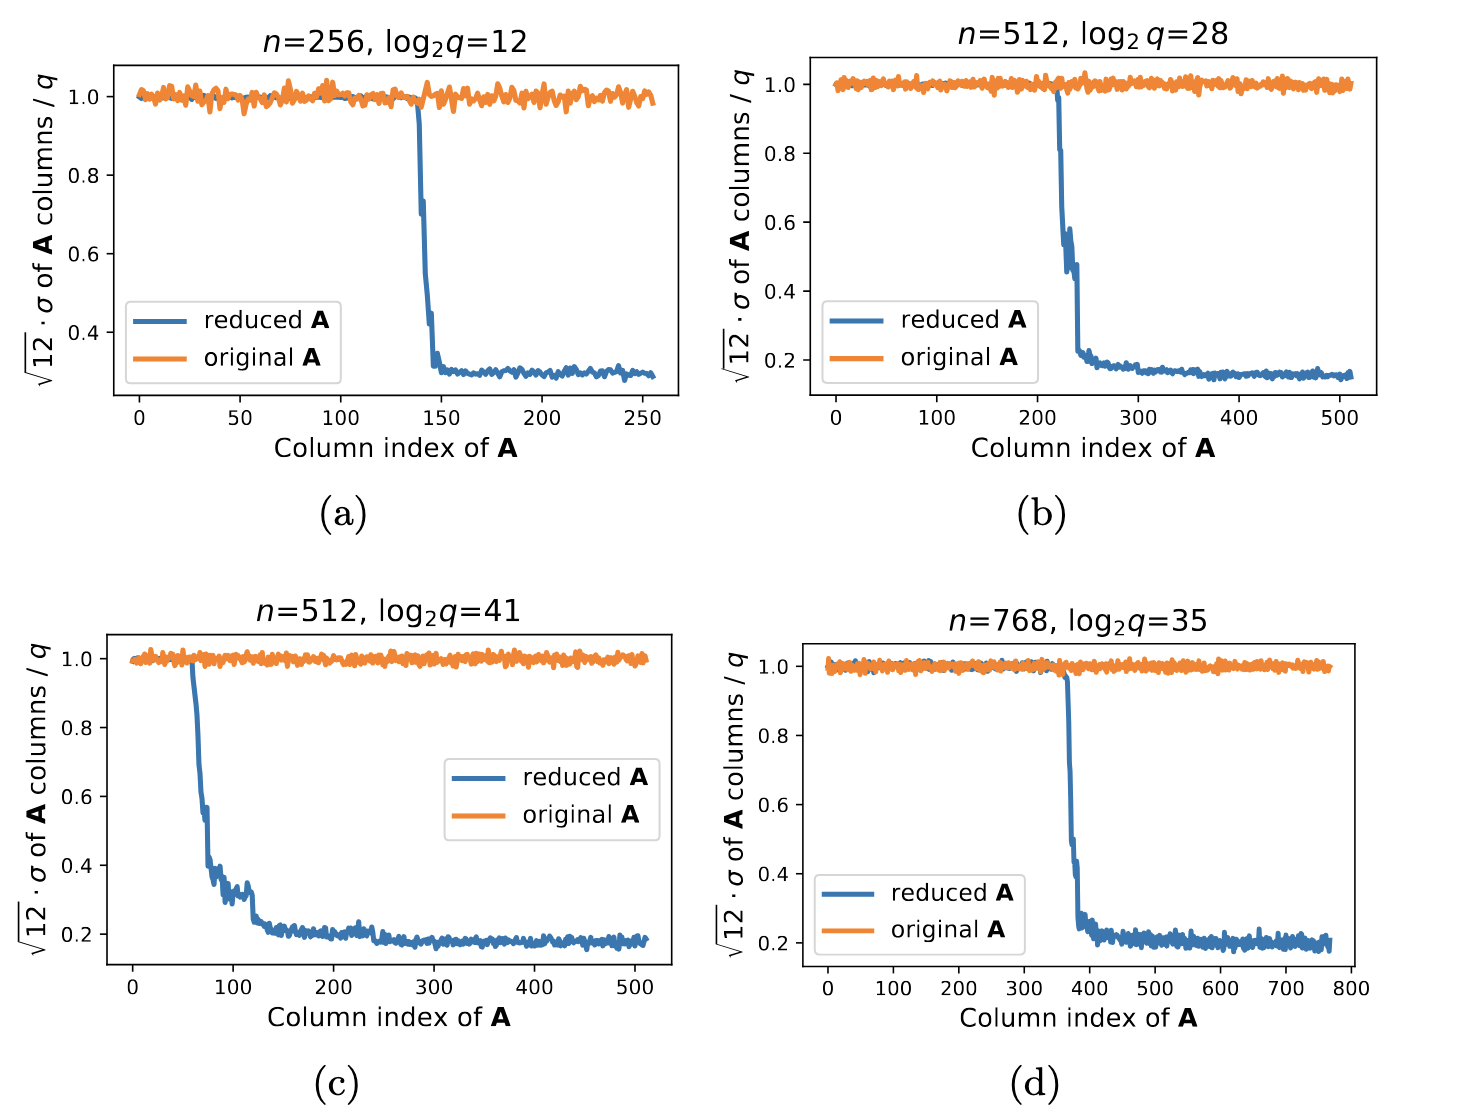
\includegraphics[width=\linewidth]{variance_slope_example.png}
  
  \scriptsize
  Empirical st.\,dev.\ profile (ex. $n\!=\!512,\;\log_2q\!=\!41$):  
  --75 = \textit{Cruel}, 75--115 = \textit{Chill}, 116-- = \textit{Cool}.  
  A visible "slope" motivates the extra middle zone. Chill reg. is up to 40b.
  
  \vspace{0.7em}
  \textbf{Key numbers (typ.\ 512‑dim):}
  \[
  \begin{aligned}
  \rho      &\approx 0.41\\
  n_{\mathrm{cruel}} &\approx 75-190\\
  n_{\mathrm{chill}} &\approx 4-40\\
  n_{\mathrm{cool}}  &\approx 150-390
  \end{aligned}
  \]
  
  \end{columns}
  
  \end{frame}
  %----------------------------------------------------  
\subsection{Outline}
%---------------------------
\begin{frame}{Broader Plan \& PhD Option}
  \begin{itemize}
    \item Continue master's thesis path, \textbf{but} preparing PhD
          application (domestic, Japan) as primary  
          {\scriptsize(Consider DC1, outsource employment, etc)}.
    \item Potential PhD topic extension:
          \begin{enumerate}
            \item Ring-LWE rotation / leakage.
            \item Adaptive defense: secret-distribution hardening.
          \end{enumerate}
  \end{itemize}
\end{frame}

%====================================================
\section{Job-Hunting Update}
%====================================================

\subsection{NTT R\&D Track}
\begin{frame}{NTT R\&D Application}
  \begin{itemize}
    \item Online entry sheet drafted; internal review this week.
    \item Next steps:
          \begin{enumerate}
            \item Submit by \textbf{end of Apr}.
            \item Expect aptitude + technical interview.
          \end{enumerate}
  \end{itemize}
\end{frame}

%---------------------------
\subsection{Other Career Paths}
\begin{frame}{Additional Employment Activities}
  \begin{itemize}
    \item \textbf{Current employer (remote dev):} negotiating long-term outsourcing
          contract through graduation; discussing possible business trips to US.
    \item Preparing 2-3 more applications (possibly consultancies / startups).
    \item Networking via conferences + LinkedIn JP market groups.
  \end{itemize}
\end{frame}

%====================================================
\section{Miscellaneous}
%====================================================

\subsection{Scholarships \& Courses}
\begin{frame}{Other Commitments}
  \begin{itemize}
    \item \textbf{Scholarships 2025:} reviewing private foundations  
          (noted on several misleading conditions).
    \item \textbf{Course load (Semester):}
          \begin{itemize}
            \item Cryptography, Soft Computing
            \item Japanese: upperintermediate/advanced, communication for business purposes
          \end{itemize}
    \item \textbf{JLPT N1} scheduled July; intensive prep.
  \end{itemize}
\end{frame}

%====================================================
\section*{Summary}
\begin{frame}{Take-aways}
  \begin{itemize}
    \item Research: hybrid \emph{Cool-Chill-Cruel} attack progressing;
          variance study + ML classifier next.
    \item Career: NTT R\&D application in final stage; parallel options open.
    \item Personal development: scholarship search, JLPT N1, 4 graduate courses.
  \end{itemize}
  \vfill
  \centering{\Large Q?}
\end{frame}

\end{document}


% ----------------------------------------------------------------------------
% TABLE OF CONTENTS
% ----------------------------------------------------------------------------
\begin{frame}{Outline}
  \tableofcontents
\end{frame}




% ----------------------------------------------------------------------------
\begin{frame}{References}
  \footnotesize
  \begin{thebibliography}{9}
    \bibitem{regev}
    O. Regev. \emph{On Lattices, Learning with Errors, Random Linear Codes, and Cryptography.} J. ACM 51(6), 2005.

    \bibitem{concrete_results}
    Niklas N., ...
    \emph{The Cool and the Cruel: Separating Hard Parts of LWE Secrets., https://eprint.iacr.org/2024/443.pdf}
    (ArXiv, 2024).
    
    \bibitem{someRef2}
    Albrecht et al. \emph{Estimate all the LWE, NTRU schemes.  https://eprint.iacr.org/2018/331} (2018).

    \bibitem{BKZ2ref}
    Chen, Y., Nguyen, P. Q.,
    \emph{BKZ 2.0: Better Lattice Security Estimates}.
    Lecture Notes in Computer Science, 2011.

    \bibitem{FlatterRef}
    Ryan, K., Heninger, N.
    \emph{Fast practical lattice reduction through iterated compression.}
    Annual International Cryptology Conference. Springer, 2023.

    \bibitem{PolishRef}
    Charton, F., Lauter, K., Li, C., Tygert, M.
    \emph{An efficient algorithm for integer lattice reduction. SIAM Journal on Matrix Analysis and Applications}
    (2024).

    \bibitem{SALSAref}
    Gama, N., Ducas, L. et al.,
    \emph{On SALSA Picante ML Attack Method. https://eprint.iacr.org/2023/340} (2023).
    % Add more references as needed
  \end{thebibliography}
\end{frame}

% ----------------------------------------------------------------------------
\end{document}
